\chapter{Retinal Fundus Image Synthesis} \label{cha:retinas}

To generate realistic retinal fundus image from the semantic labels, we use an image-to-image translation network.

\section{SPADE}

\begin{figure}[h]
    \centering
    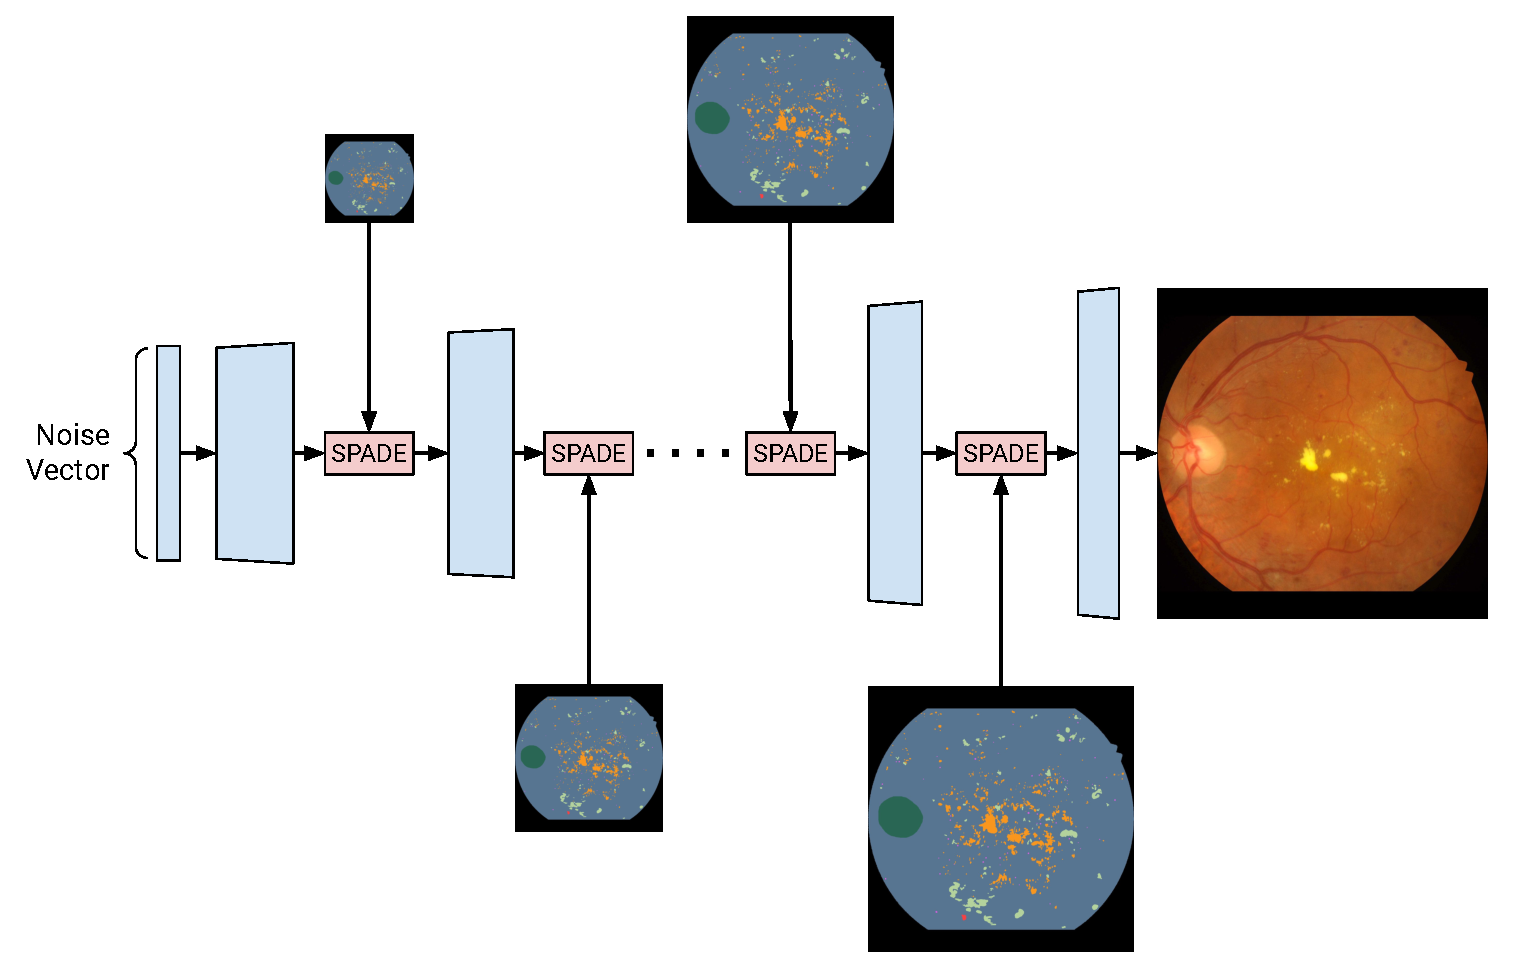
\includegraphics[width=\textwidth]{retinas/figs/spade-arch.pdf}
    \caption{Illustration of how the SPADE generator is conditioned.}
    \label{fig:spadearch}
\end{figure}

Spatially-Adaptive (De)normalisation (SPADE) is a conditional normalisation layer, like AdaIN\footnote{Interestingly, other conditional normalisation techniques such as AdaIN are actually special cases of SPADE.}, but specially crafted for the semantic image synthesis task \cite{spade}.
In SPADE, the parameters $\gamma$ and $\beta$ are now tensors instead of vectors as in AdaIN or batch normalisation. Once again, consider $X \in \mathbb{R}^{N\times C\times H\times W}$ and also the segmentation mask $M \in \mathbb{L}^{H\times W}$ where $\mathbb{L}$ is a set of integers representing the labels present in the mask. Then the SPADE transform is given by
\begin{align}
    \text{SPADE}(X, M) = \gamma_{chw}(M) \left( \frac{ X_{nchw} - \mu_c(X)}{\sigma_c(X)} \right) + \beta_{chw}(M)
\end{align}
where $\mu_c, \sigma_c$ are defined in the same way as in batch normalisation (\Cref{eq:bnmean} and \eqref{eq:bnstd}), and $\gamma_{chw}, \beta_{chw}$ denote functions that convert the segmentation map $M$ to the scalar denormalisation parameters. In practice, these functions are implemented as small convolutional networks.

Since the denormalisation parameters themselves encode enough information about the label map, we are able to discard the entire encoder part of the network in the SPADE generator.
Instead, we pass the resized segmentation map directly to the SPADE layers in the generator network, 
as depicted in \Cref{fig:spadearch}.
Note the similarity with StyleGAN in that they both inject information into conditional normalisation layers, whereas traditional GAN architectures feed information forward from the first layer.

We use the same multi-scale discriminator used in pix2pixHD.
The network is trained to translate semantic labels of resolution $512\times512$ to realistic retinal fundus images of the same size.
Weights are initialised using Xavier initialisation, and we use Hinge loss as our loss function.

Additional information is provided to the model in the form of optic disc instance maps.
Apart from these and the semantic labels, we do not provide any other form of conditioning, such as grading information.

\section{Experiments}

Experiments with this network were much more limited due to long training times and limited access to hardware.

We use the Adam optimiser with $\alpha_G = \alpha_D = 0.0002$, $\beta_1 = 0.0$, $\beta_2 = 0.9$, and a latent dimension of 256.
The network was trained for 500 epochs on two GPUs over 182 hours.

\begin{figure}[h]
    \centering
    \begin{subfigure}{0.40\textwidth}
        \centering
        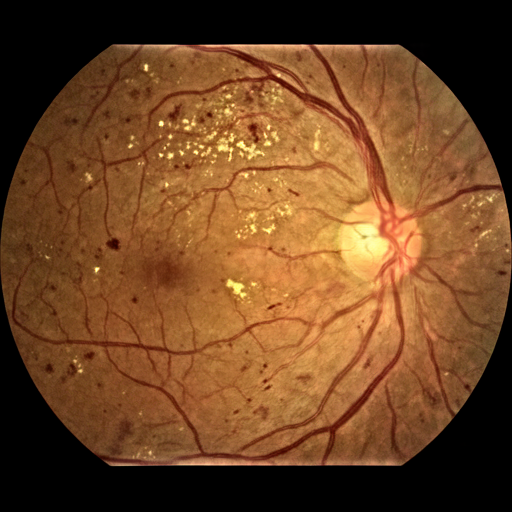
\includegraphics[width=\linewidth]{retinas/figs/no_inst.png}
        \caption{Without instance map.}
        \label{fig:without_inst}
    \end{subfigure} %
    \begin{subfigure}{0.40\textwidth}
        \centering
        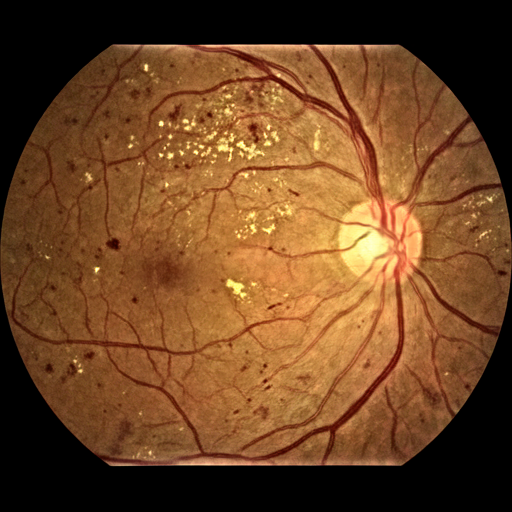
\includegraphics[width=\linewidth]{retinas/figs/with_inst.png}
        \caption{With instance map.}
        \label{fig:with_inst}
    \end{subfigure}
    \caption{Effect of instance maps.}
    \label{fig:with_without_instance}
\end{figure}

We found that the network was capable of producing realistic retina texture and structures, including blood vessels and the macula (the dark circle opposite the optic disc).
This is impressive, considering that there is no guidance for retinal structures in the semantic labels.
The network is also able to accurately place the lesions according to the semantic labels.

Layout prediction of the optic disc in particular was important for visually plausible retinas, as we found that without providing explicit conditioning in the form of instance maps the SPADE generator created images which exhibited optic discs with poorly defined boundaries.
This can be seen in \Cref{fig:with_without_instance}, where without an instance map, the optic disc is blurry and the vessels display more inconsistencies.

\subsection{Samples}

The resulting images show good diversity, with the ability to the generate different lighting conditions that were present in the source data.
A sample of images are shown in \Cref{fig:spade_sample}.

\begin{figure}[h]
    \centering
    \begin{subfigure}{0.3\textwidth}
        \centering
        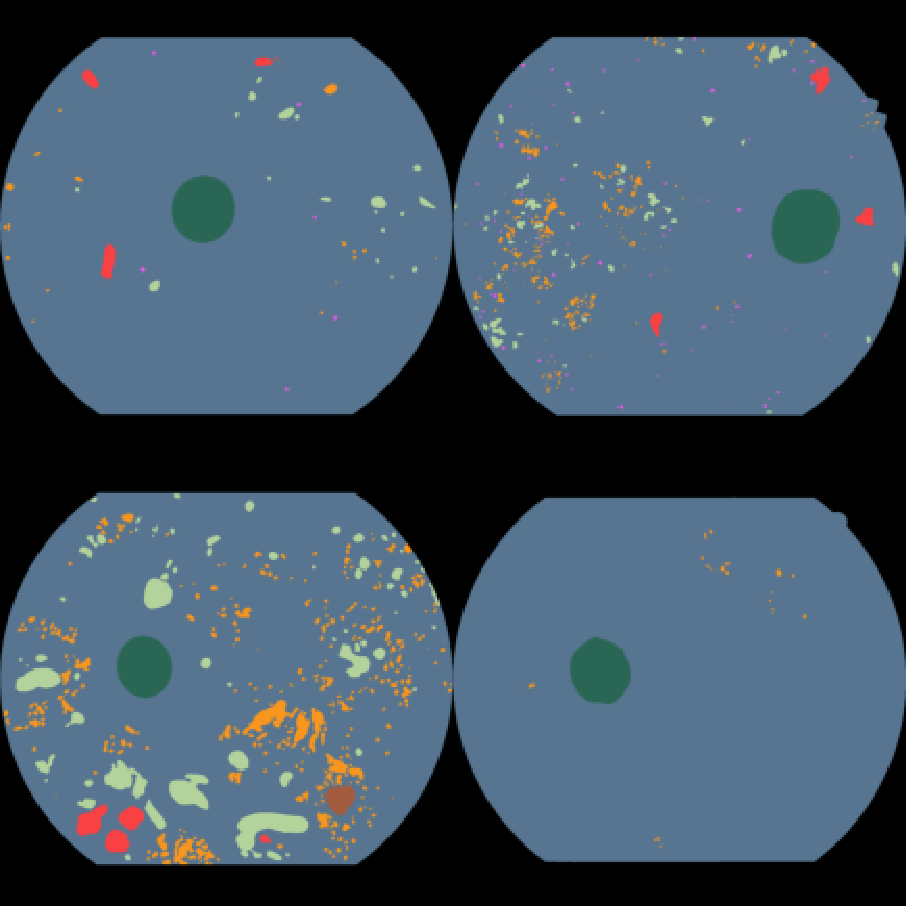
\includegraphics[width=\linewidth]{retinas/figs/spade_good_sample_labels.pdf}
        \caption{Real semantic labels.}
        \label{fig:spade_label_sample}
    \end{subfigure}
    \begin{subfigure}{0.3\textwidth}
        \centering
        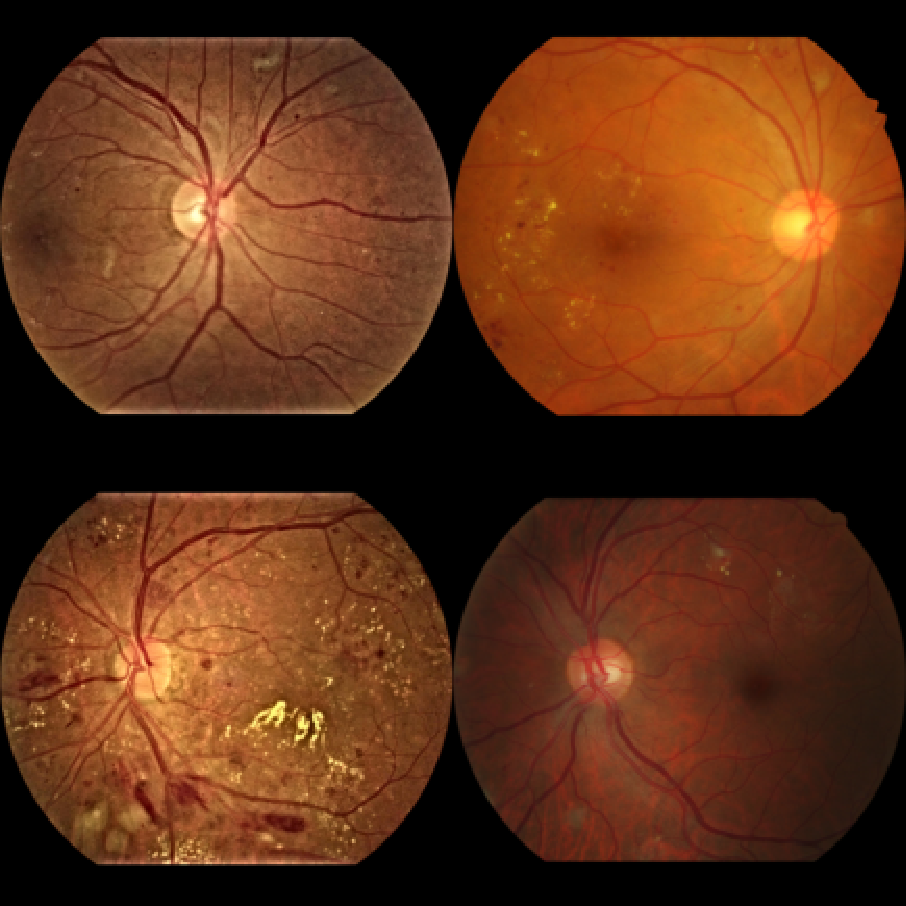
\includegraphics[width=\linewidth]{retinas/figs/spade_good_sample_images.pdf}
        \caption{Real images.}
        \label{fig:spade_image_sample}
    \end{subfigure}
    \begin{subfigure}{0.3\textwidth}
        \centering
        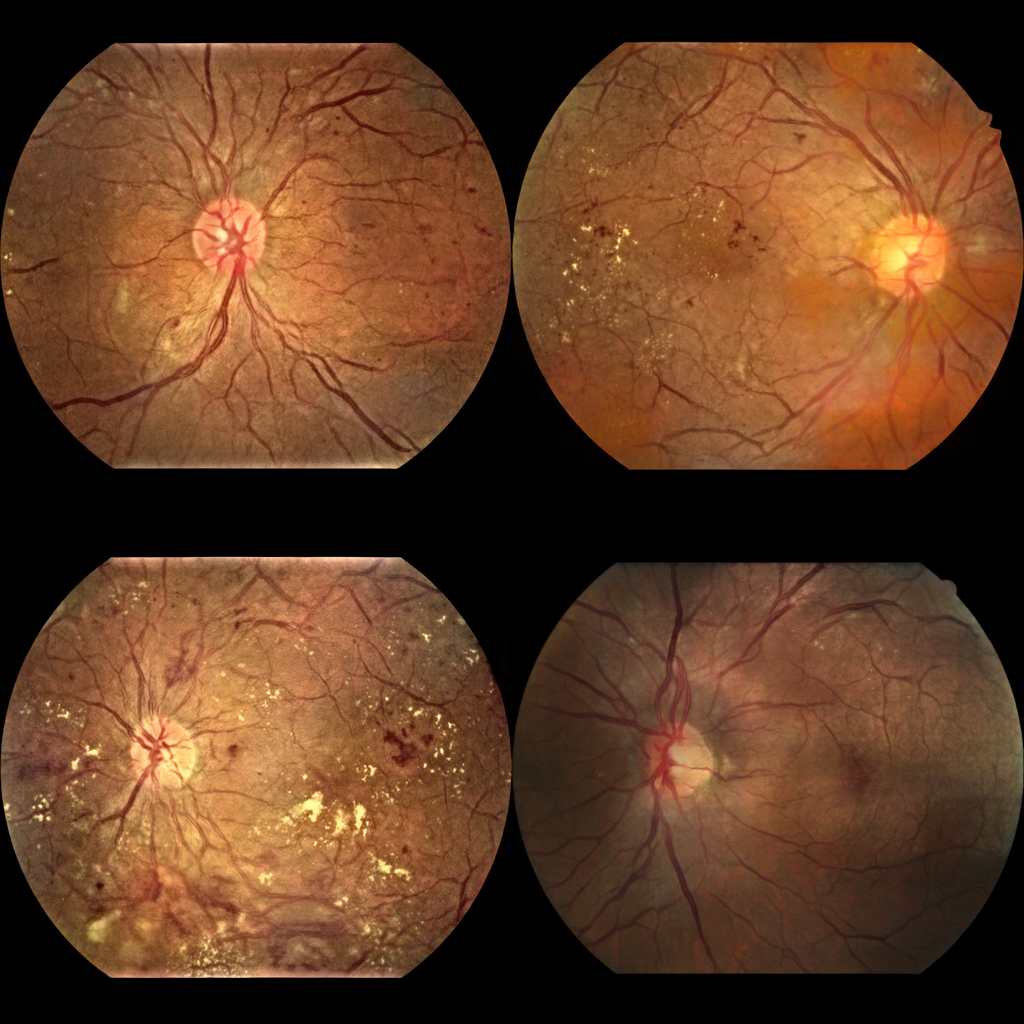
\includegraphics[width=\linewidth]{retinas/figs/spade_sample1.png}
        \caption{SPADE output.}
        \label{fig:spade_generated_sample}
    \end{subfigure}
    \caption{Comparison of real images and SPADE outputs for semantic labels from the validation set.}
    \label{fig:spade_sample}
\end{figure}

\subsection{Common Failure Modes}

\begin{figure}[h]
    \centering
    \begin{subfigure}{0.40\textwidth}
        \centering
        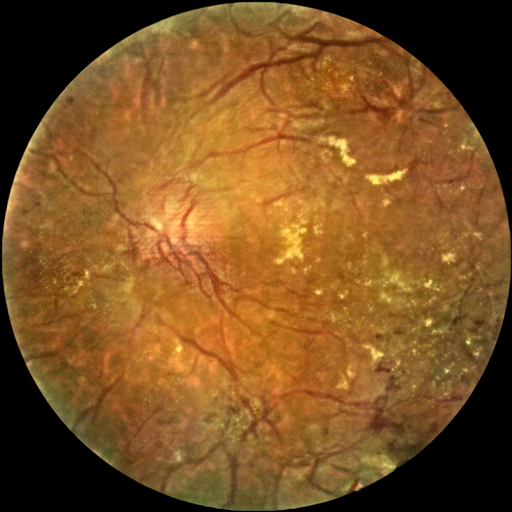
\includegraphics[width=\linewidth]{retinas/figs/no-od.png}
        \caption{Generated image with a misplaced vascular root.}
        \label{fig:no_od}
    \end{subfigure}
    \begin{subfigure}{0.40\textwidth}
        \centering
        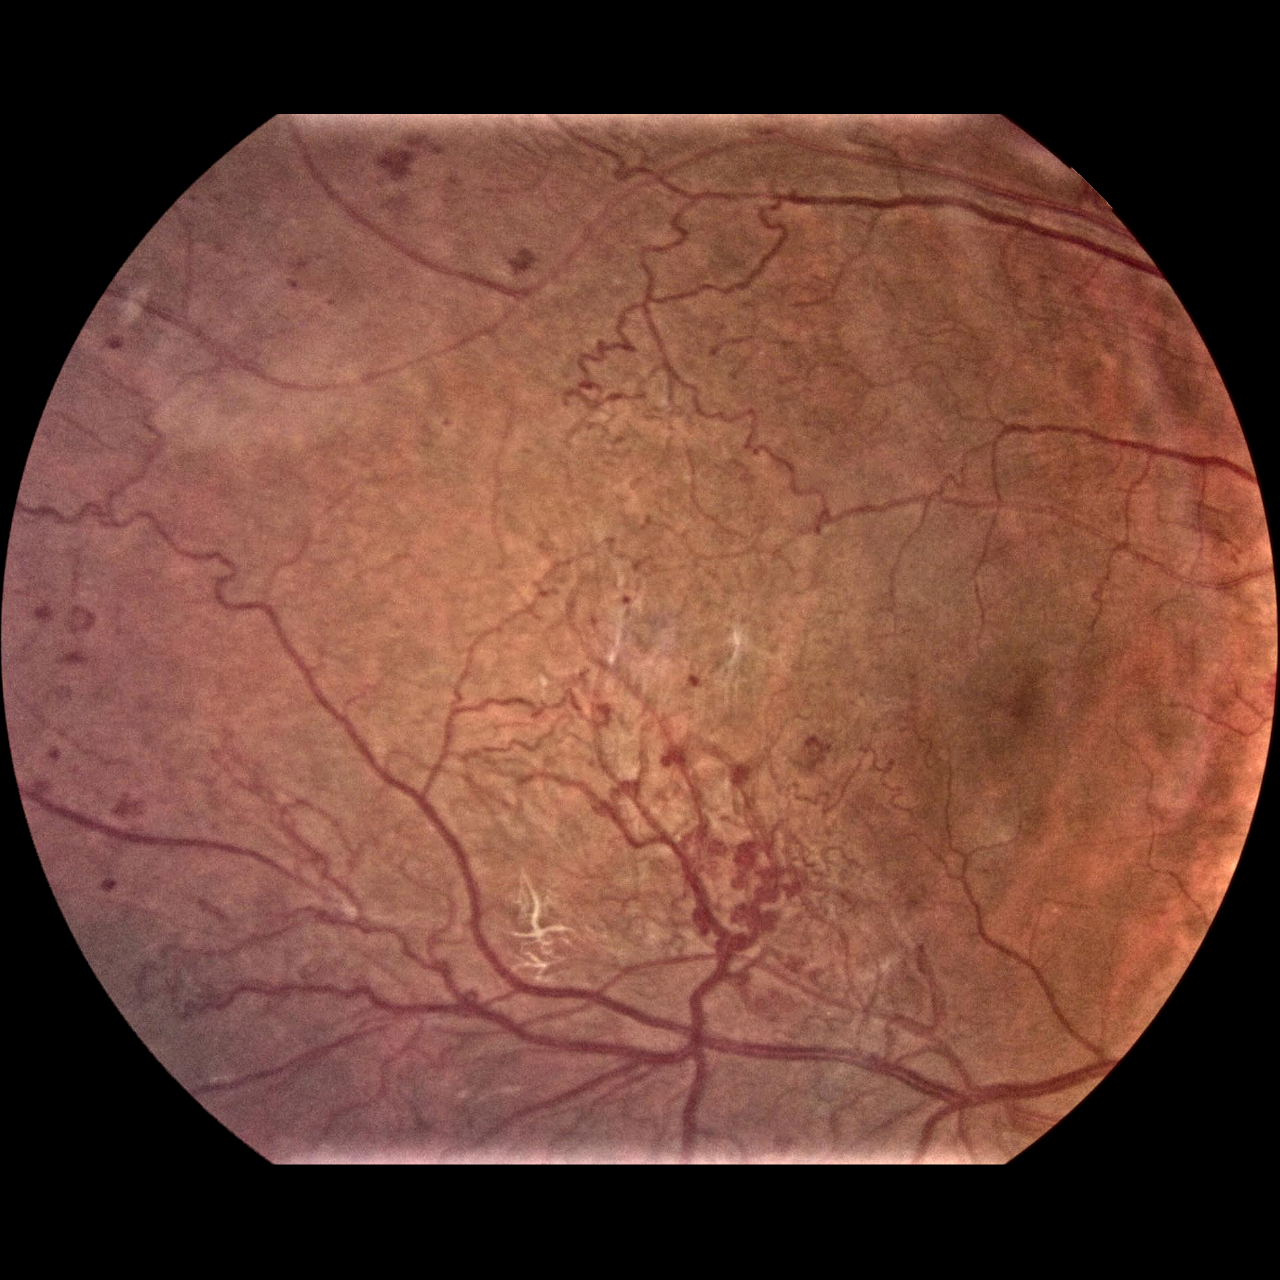
\includegraphics[width=\linewidth]{retinas/figs/no-od-real.png}
        \caption{Real photograph with obscured optic disc.}
        \label{fig:no_od_real}
    \end{subfigure}
    \caption{Examples of common failure modes.}
    \label{fig:spade_bad_sample}
\end{figure}

\begin{description}
    \item[Misplaced Vascular Root] \hfill \\
    When the optic disc is not present in the semantic label, the network has difficulty placing the vascular ``root''.
    Example shown in \Cref{fig:no_od}.
    It is possible that the optic disc is obscured in a real retinal fundus photograph, as in \Cref{fig:no_od_real}, however there are only two examples of this in the training set, and the network is unable to infer that the vascular root should exist elsewhere.
    
    \item[Unrealistic Vascular Structure] \hfill \\
    Even when the optic disc is not occluded, the network sometimes generates unrealistic retinal vasculature, with non-contiguous regions.
    
    \item[Blurriness] \hfill \\
    In general, the images appear blurrier at smaller scales than the real photographs, which are sharp.
    Again, this is particularly apparently when examining the blood vessels in detail.
\end{description}

\subsection{Results}

Similarly to before, we compute the FID between the target dataset and the real training set, with results shown in \Cref{tab:spade_validation}.
The synthetic images are generated by providing SPADE with the real validation semantic labels as input to produce fake retinal fundus images as output.
Again, we also provide the FID score on the real validation retinal fundus photographs as a baseline.
We compare the original retinal fundus images, without applying illumination correction.

\begin{table}[h]
    \centering
    \begin{tabular}{lr}
        \toprule
        Configuration & FID$\downarrow$ \\
        \midrule
        Validation & 23.491 \\
        \midrule
        SPADE & 48.438 \\
        + instance maps & \textbf{46.603} \\
        \bottomrule
    \end{tabular}
    \caption{FID scores between real images from the training set and the output of SPADE on the real validation semantic labels. Best results for each metric in bold (excluding the baseline).}
    \label{tab:spade_validation}
\end{table}

This shows that the use of instance maps yield a small improvement in overall image quality.
Unfortunately, since we are not able to obtain the code for DR-GAN or Tub-sGAN, and since the authors did not state the dimensionality used to compute the FID scores reported in their papers (which can alter the score by orders of magnitude), it's impossible to draw a quantitative comparison.
Instead, we leave this as future work.
